% \tikzset{%
%   every neuron/.style={
%     circle,
%     draw,
%     minimum size=1cm
%   },
%   neuron missing/.style={
%     draw=none, 
%     scale=4,
%     text height=0.333cm,
%     execute at begin node=\color{black}$\vdots$
%   },
% }
\begin{figure}[H]
  \centering

  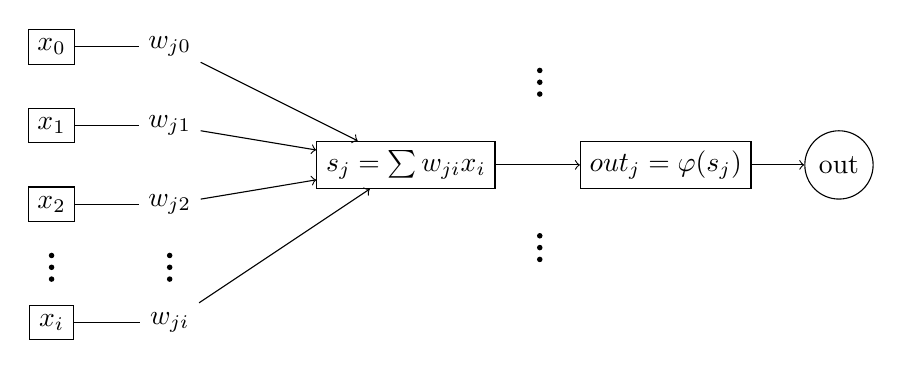
\begin{tikzpicture}
    \tikzstyle{rectangle_style}=[rectangle, draw]
    \tikzstyle{dividedrectangle_style}=[draw, rectangle split, rectangle split parts=2, rotate = 90, minimum height = 15mm, minimum width = 10mm]
    
    % neuron i
    \foreach \x in {0,...,2}
      \draw node at (0, -\x) [rectangle_style] (neuron_i_\x) {$x_\x$};
    \foreach \x in {1,...,3}
      \fill (0, -2.5 - \x*0.15) circle (1pt);
    \draw node at (0, -3.5) [rectangle_style] (neuron_i_3) {$x_i$};
    
    % w_ji
    \foreach \x in {0,...,2}
      \draw node at (1.5, -\x) [] (w_ji_\x) {$w_{j\x}$};
    \draw node at (1.5, -3.5) [] (w_ji_i) {$w_{ji}$};
    \foreach \x in {1,...,3}
      \fill (1.5, -2.5 - \x*0.15) circle (1pt);
    
    % neuron sum
    \draw node at (4.5, -1.5) [rectangle_style] (neuron_sum) {
      $s_j = \sum {w_{ji}x_i}$
    };
    \draw node at (7.8, -1.5) [rectangle_style] (neuron_act) {
      $out_j = \varphi (s_j)$
    };
    \foreach \x in {1,...,3}
      \fill (6.2, -2.25 - \x*0.15) circle (1pt);
    \foreach \x in {1,...,3}
      \fill (6.2,  - 0.15 - \x*0.15) circle (1pt);
    
    % output
    \node at (10, -1.5) [circle, draw] (output) {out};    

    
    % connect: y_i -> w_ji
    \foreach \i in {0,...,2}
      \path[-] (neuron_i_\i) edge node[] {} (w_ji_\i);
    \path[-] (neuron_i_3) edge node[] {} (w_ji_i);
    
    % connect: w_ji -> neuron j
    \foreach \i in {0,...,2}
      \path[->] (w_ji_\i) edge node[] {} (neuron_sum);
    \path[->] (w_ji_i) edge node[] {} (neuron_sum);
    
     % connect: neuron sum  -> neuron act
     \path[->] (neuron_sum) edge node[above, midway] {$ $} (neuron_act);

    % connect: neuron act -> output
    \path[->] (neuron_act) edge node[above, midway] {$ $} (output);

    
  \end{tikzpicture}
\caption{Схема искуственного нейрона} \label{simple-neuron}
\end{figure}